\documentclass[tikz, border=5mm]{standalone}
\usepackage{tikz}
\usetikzlibrary{shapes.geometric, arrows.meta, positioning}

\begin{document}
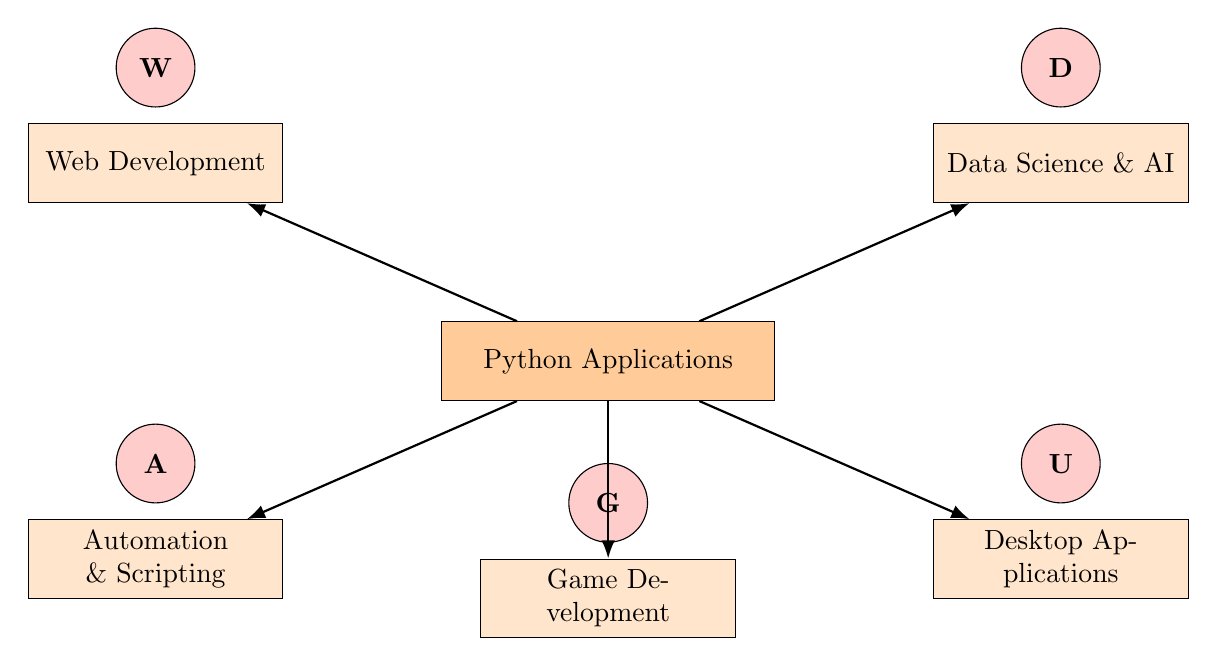
\begin{tikzpicture}[
    node distance=1.5cm,
    app/.style={rectangle, draw, fill=orange!20, text width=3cm, text centered, minimum height=1cm},
    icon/.style={circle, draw, fill=red!20, minimum size=1cm, inner sep=0pt, font=\bfseries},
    arrow/.style={-Latex, thick}
]

% Central node
\node (python) at (0,0) [app, fill=orange!40, text width=4cm] {Python Applications};

% Application nodes with icons
\node (web_dev) [app, above left=1.5cm and 2cm of python] {Web Development};
\node (icon_web) [icon, above=2mm of web_dev] {W};
\node (data_ai) [app, above right=1.5cm and 2cm of python] {Data Science \& AI};
\node (icon_data) [icon, above=2mm of data_ai] {D};

\node (automation) [app, below left=1.5cm and 2cm of python] {Automation \& Scripting};
\node (icon_auto) [icon, above=2mm of automation] {A};
\node (desktop) [app, below right=1.5cm and 2cm of python] {Desktop Applications};
\node (icon_desktop) [icon, above=2mm of desktop] {U};

\node (game_dev) [app, below=2cm of python] {Game Development};
\node (icon_game) [icon, above=2mm of game_dev] {G};

% Connections
\draw [arrow] (python) -- (web_dev);
\draw [arrow] (python) -- (data_ai);
\draw [arrow] (python) -- (automation);
\draw [arrow] (python) -- (desktop);
\draw [arrow] (python) -- (game_dev);

\end{tikzpicture}
\end{document}
